\section{Extended Related Work}

\subsection{Agent Memory}

A growing body of work explores how agents can accumulate experience from past trajectories and leverage external (often non-parametric) memory to guide future actions. 
AgentFly~\citep{zhou2025agentfly} presents an extensible framework where memory evolves continuously as agents solve tasks, enabling scalable reinforcement learning and long-horizon reasoning across diverse environments. 
AWM (Agent Workflow Memory)~\citep{wang2024agent} induces reusable \emph{workflows}, \ie structured routines distilled from past trajectories, and selectively injects them into memory to improve efficiency and generalization in web navigation benchmarks. 
A-MEM~\citep{xu2025mem} introduces a dynamically organized memory system inspired by the Zettelkasten method: each stored memory is annotated with structured attributes (\eg tags, keywords, contextual descriptions) and automatically linked to relevant past entries, while existing entries are updated to integrate new knowledge, yielding adaptive and context-aware retrieval. 
Agentic Plan Caching~\citep{zhang2025cost} instead focuses on cost efficiency by extracting reusable plan templates from agent trajectories and caching them for fast execution at test time. 

Together, these works demonstrate the value of external memory for improving adaptability, efficiency, and generalization in LLM agents. 
Our work differs by tackling the broader challenge of \emph{context adaptation}, which spans not only agent memory but also system prompts, factual evidence, and other inputs underpinning AI systems. 
We further highlight two fundamental limitations of existing adaptation methods: \textit{brevity bias} and \textit{context collapse}; and show that addressing them is essential for robustness, reliability, and scalability beyond raw task performance. 
Accordingly, our evaluation considers not only accuracy but also cost, latency, and scalability.

\section{Extended Discussions}

\subsection{ACE vs. GEPA}
\textbf{Scope and Objective}
Both GEPA and ACE improve model or agent behavior by adapting \emph{context} at test time (rather than updating model weights), but they are designed for different forms of adaptation.
GEPA treats adaptation as \emph{prompt evolution}: it iteratively proposes and selects improved instruction prompts using rollout trajectories and reflective feedback, aiming to maximize a task evaluator under a rollout budget.
ACE targets settings where performance depends on accumulating and preserving \emph{many granular, reusable insights} over long horizons.
For multi-turn agents (\eg AppWorld), the model must retain step-by-step procedures and tool-use rules across an interaction.
For domain-specific and knowledge-intensive benchmarks (\eg FiNER, Formula), accuracy depends on keeping many specific rules, edge cases, and domain concepts that are difficult to compress into a single instruction prompt without losing detail.

\textbf{Update Mechanism and Representation}
GEPA updates context by generating and selecting \emph{new prompt variants} in an evolutionary loop, where each candidate is a full prompt optimized end-to-end. 
ACE instead represents context as a structured, itemized Playbook and applies \emph{incremental delta updates}: the Curator writes only the new insight, and we merge it into the Playbook with simple deterministic logic. 
This avoids repeated full-prompt rewrites, helps keep earlier rules stable over long runs, and enables fine-grained bookkeeping (\eg de-duplication, targeted refinement, and tracking which entries helped or harmed accuracy). 

\subsection{ACE vs. Dynamic Cheatsheet (DC)} 
\textbf{Scope and Objective}  
Both DC and ACE collect reusable insights at test time, but they are aimed at different settings.
DC is mainly evaluated on single-turn reasoning benchmarks (\eg AIME, Game-of-24, GPQA) where each query is independent. In this regime, improvements often come from saving short, reusable heuristics and executable artifacts (\eg code snippets) that help on later problems.
ACE focuses on settings where the details and high-fidelity guidenace need to stick around. 
For multi-turn agents (\eg AppWorld), the model must remember step-by-step procedures and tool-use rules across an interaction. 
For domain-specific and knowledge-intensive benchmarks (\eg FiNER, Formula), accuracy depends on keeping many specific rules, edge cases, and domain concepts, which are hard to compress without losing information.

\textbf{Update Mechanism} 
DC updates its memory by rewriting the cheatsheet as a whole, either by regenerating the full cheatsheet each step (DC-CU) or by writing a new summary from retrieved examples (DC-RS).
With repeated full rewrites, the model tends to shorten and compress what was written before.
This can cause context collapse, which means that useful domain-specific details get dropped over time or disappear suddenly (\S\ref{subsec:limitations}).
ACE avoids full rewrites by using incremental delta updates. 
The Curator only writes the new insight, and we merge it into a structured and itemized Playbook with simple deterministic logic. 
This keeps earlier rules stable over long runs and also makes it easier to track which items helped, remove duplicates, and refine entries. 
In our ablations (\S\ref{subsec:results-ablation}), removing delta updates leads to a large drop on AppWorld (-11.7\% TGC and -27.8\% SGC on test-normal), showing that delta updates are a core part of our method.

\section{AppWorld Leaderboard Snapshot (09/2025)}
\label{subsec:appworld-leaderboard}

\begin{figure}[htbp]
    \centering
    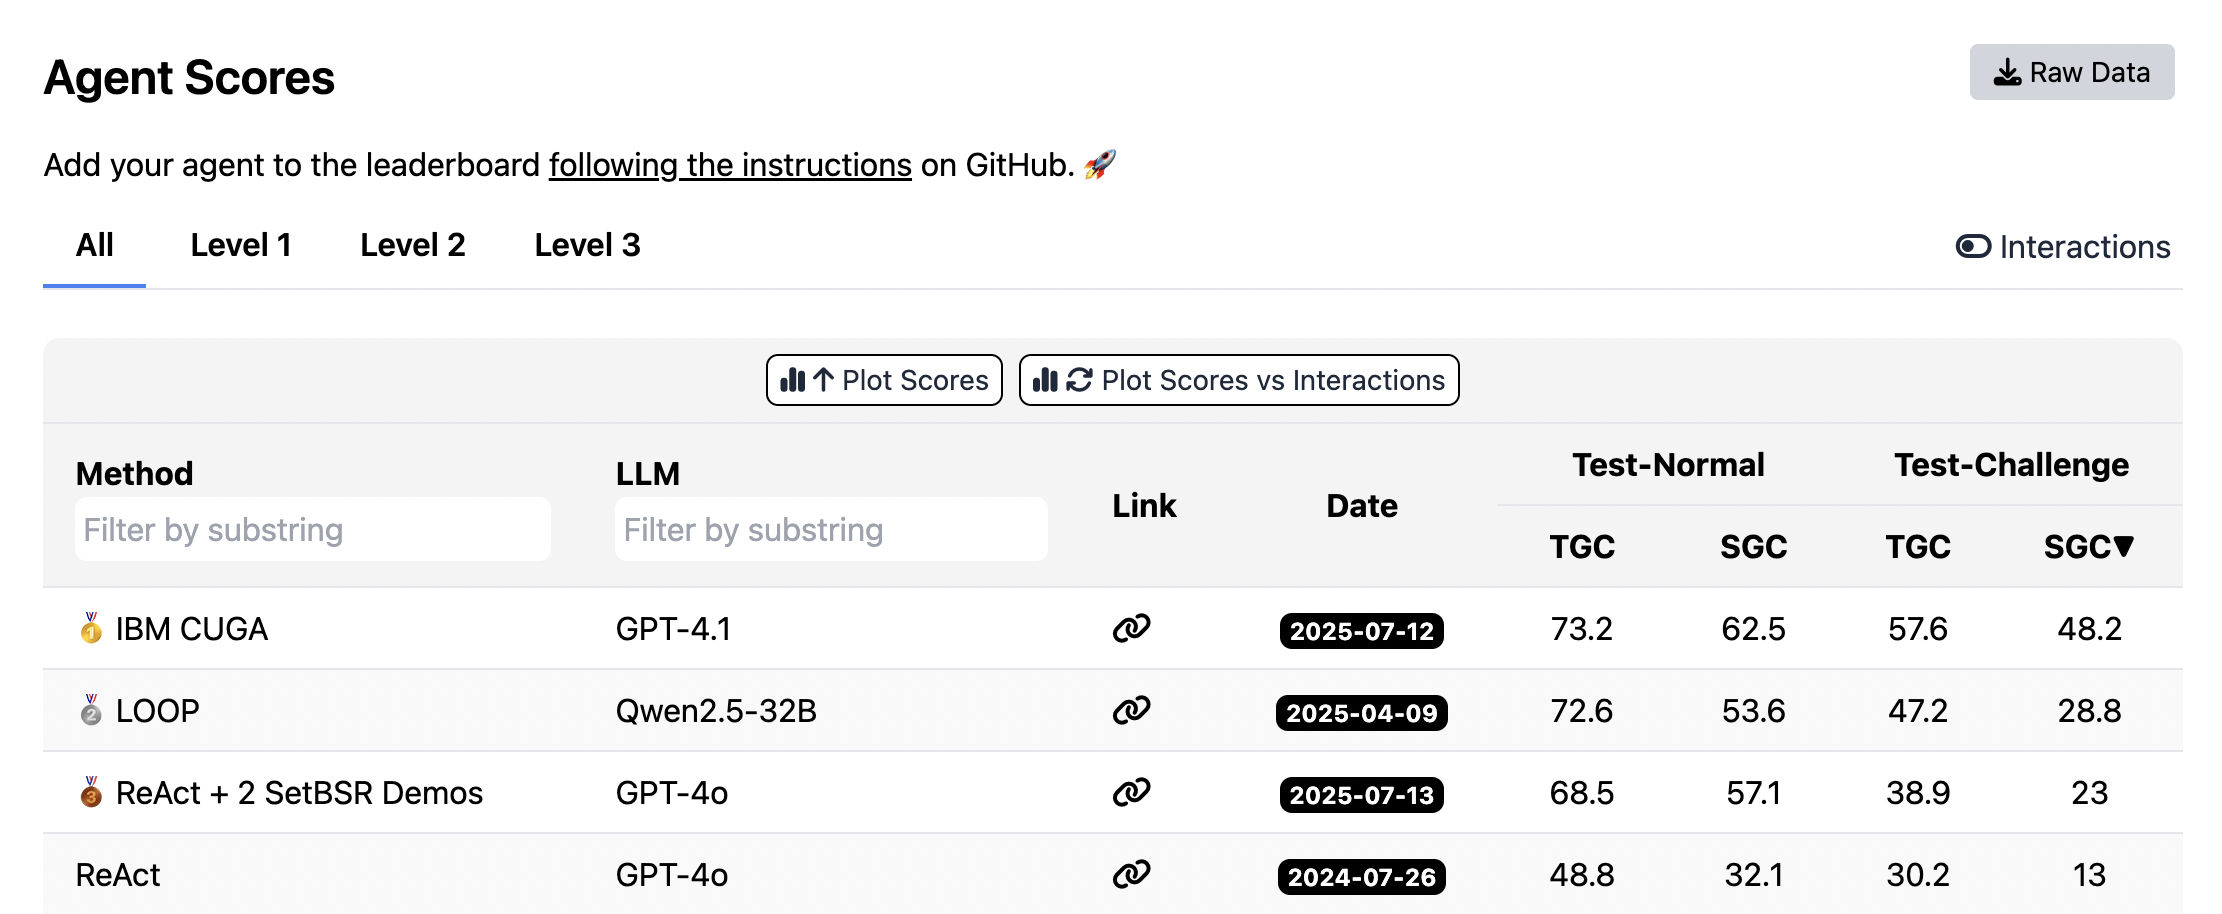
\includegraphics[width=0.8\textwidth]{figures/figure_5_CR.png}
    \caption{The AppWorld leaderboard as accessed on 09/2025.}
    \label{fig:appworld-leaderboard}
\end{figure}

\section{The Use of Large Language Models (LLMs)}

This work focuses on developing algorithms and system frameworks for effective context adaptation in large language models (LLMs). 
Accordingly, our experiments employ LLMs for the empirical evaluation of the proposed methods. 
For paper preparation, we used LLMs only to polish writing (\eg correcting grammatical errors), and not to generate new text from scratch.

\newpage
\section{Prompts}


\begin{figure}[htbp]
    \centering
    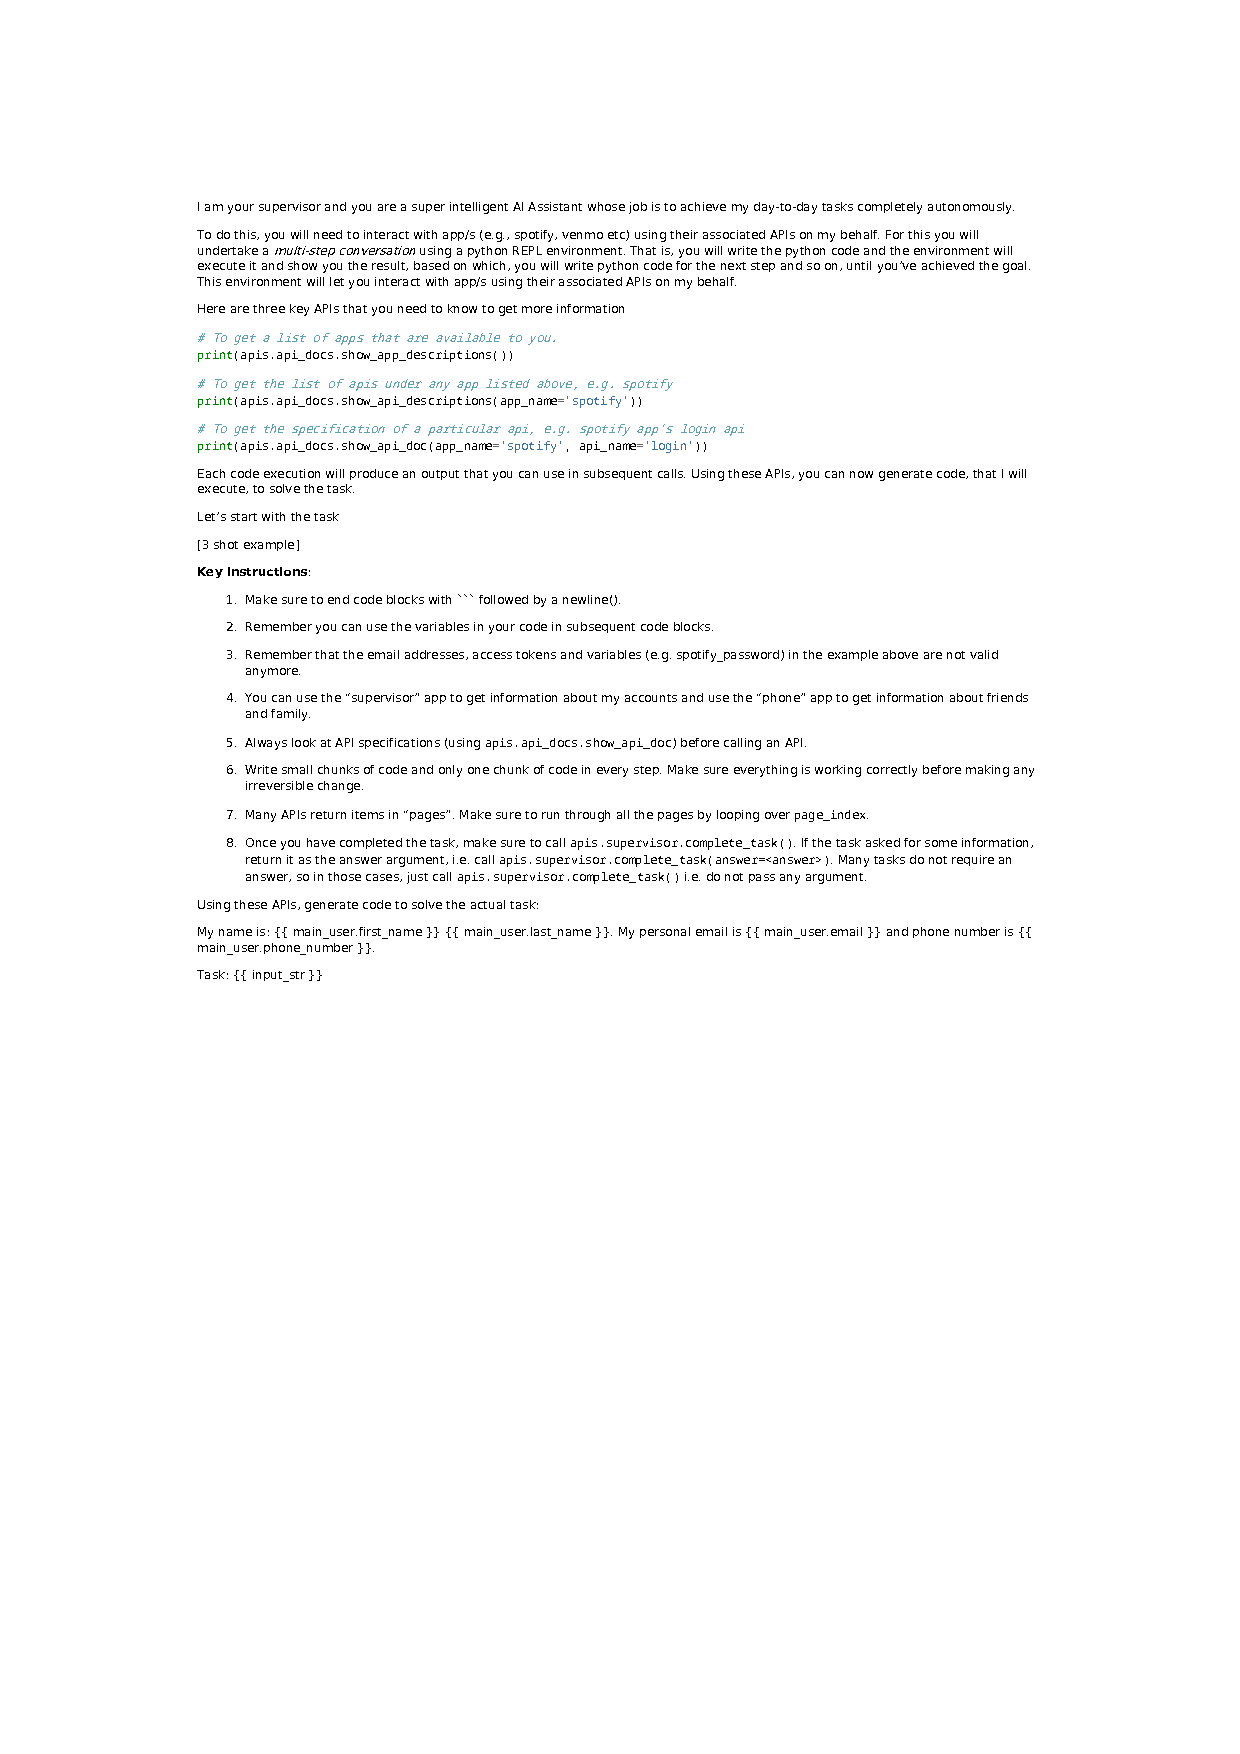
\includegraphics[width=\textwidth]{figures/prompts/icl_prompt_2.pdf}
    \caption{ICL-baseline Generator prompt on AppWorld}
    \label{fig:icl_prompt}
\end{figure}

\begin{figure}[htbp]
    \centering
    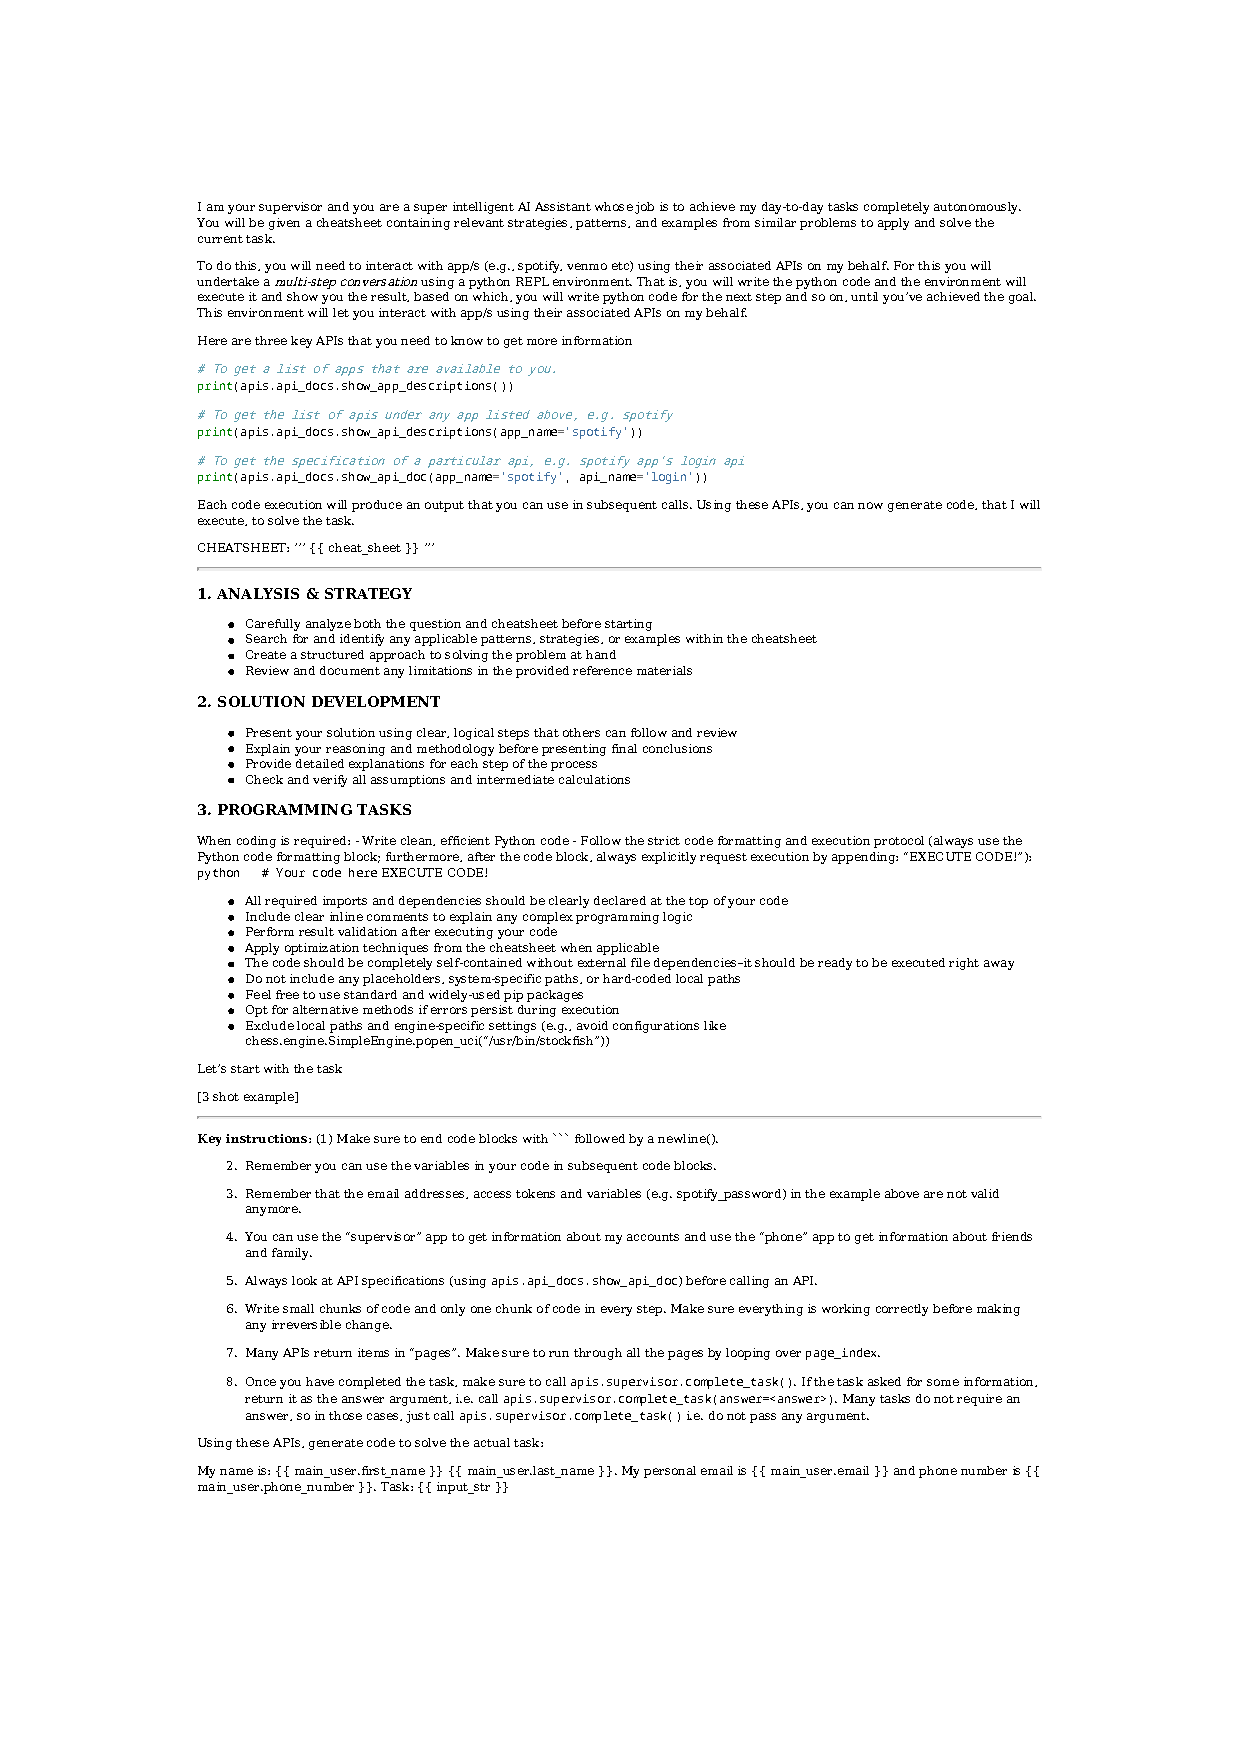
\includegraphics[width=\textwidth]{figures/prompts/DC_prompt.pdf}
    \caption{Dynamic Cheatsheet Generator prompt on AppWorld}
    \label{fig:icl_prompt}
\end{figure}

\begin{figure}[htbp]
    \centering
    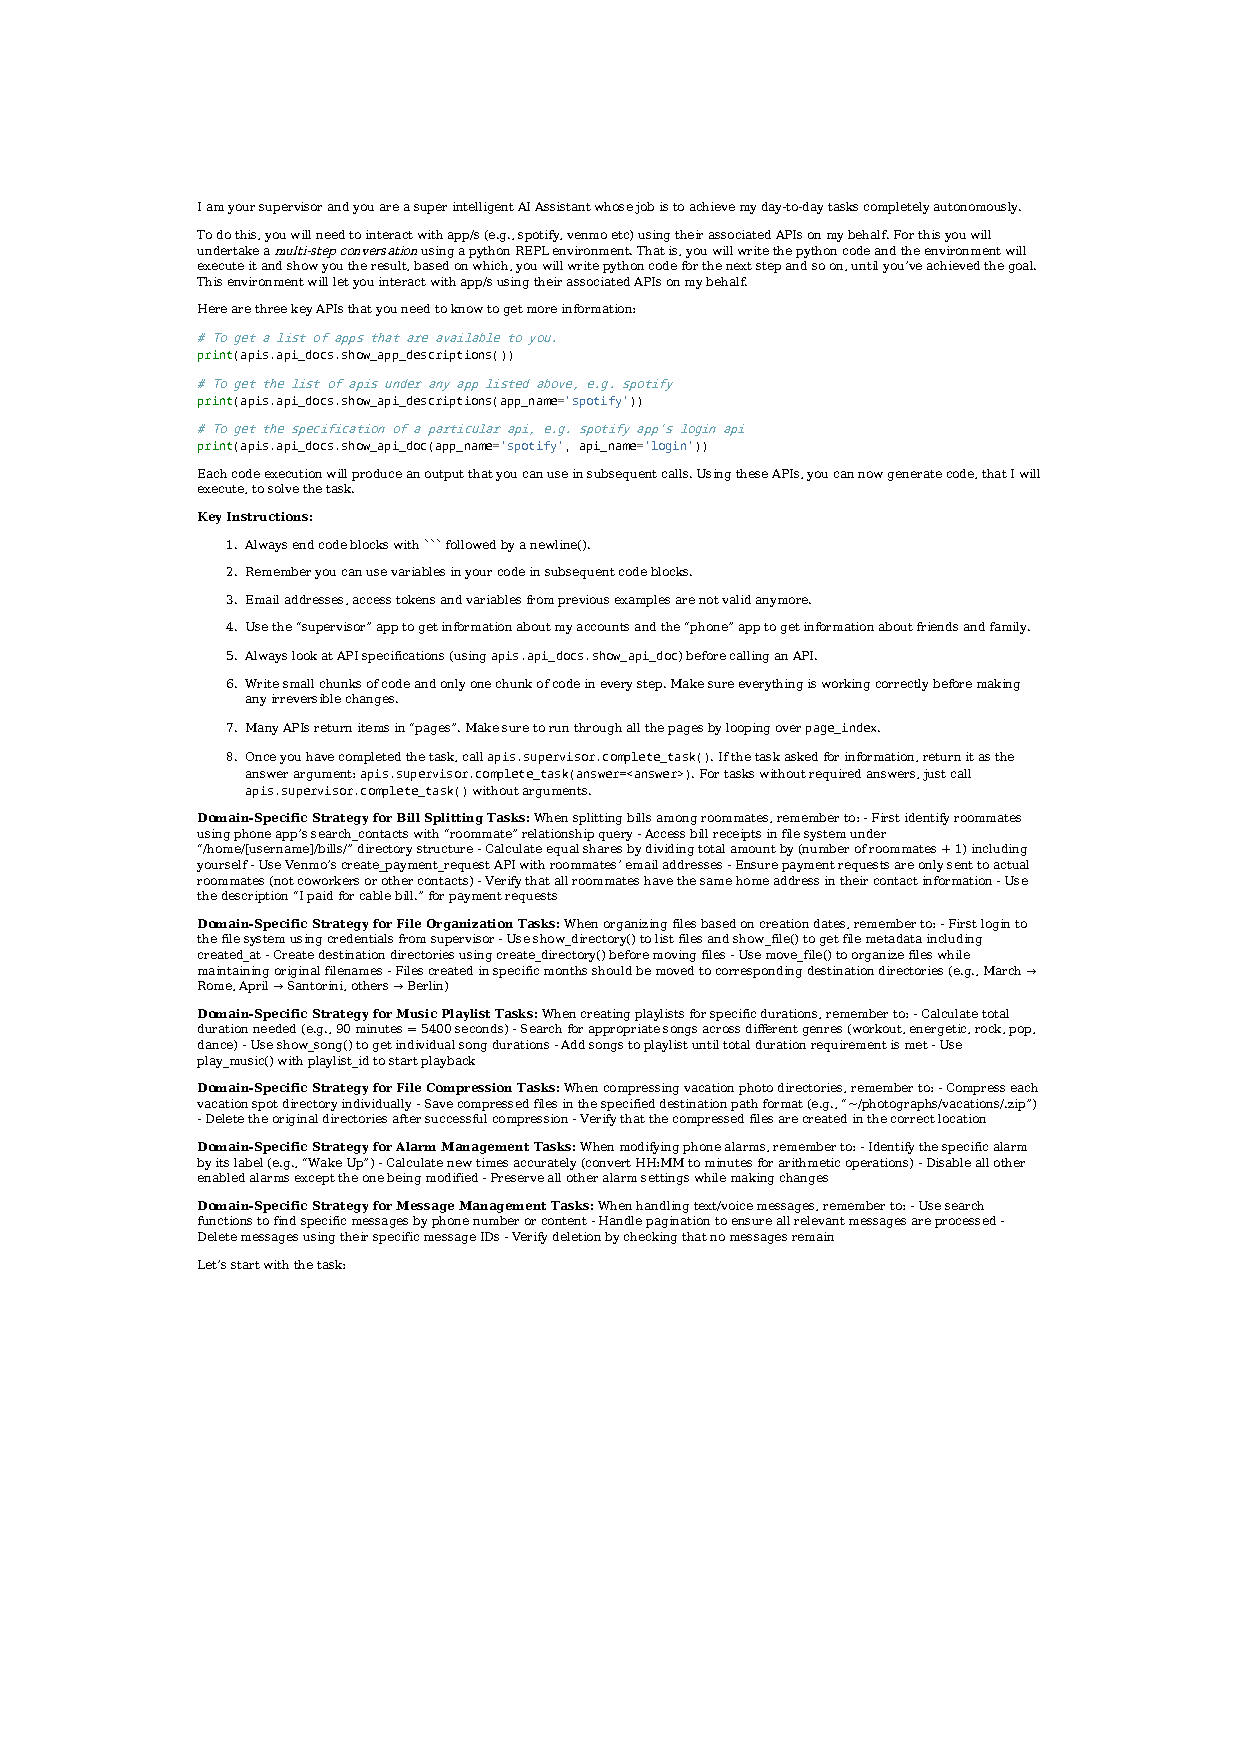
\includegraphics[width=\textwidth]{figures/prompts/gepa_prompt.pdf}
    \caption{GEPA prompt on AppWorld}
    \label{fig:icl_prompt}
\end{figure}

\begin{figure}[htbp]
    \centering
    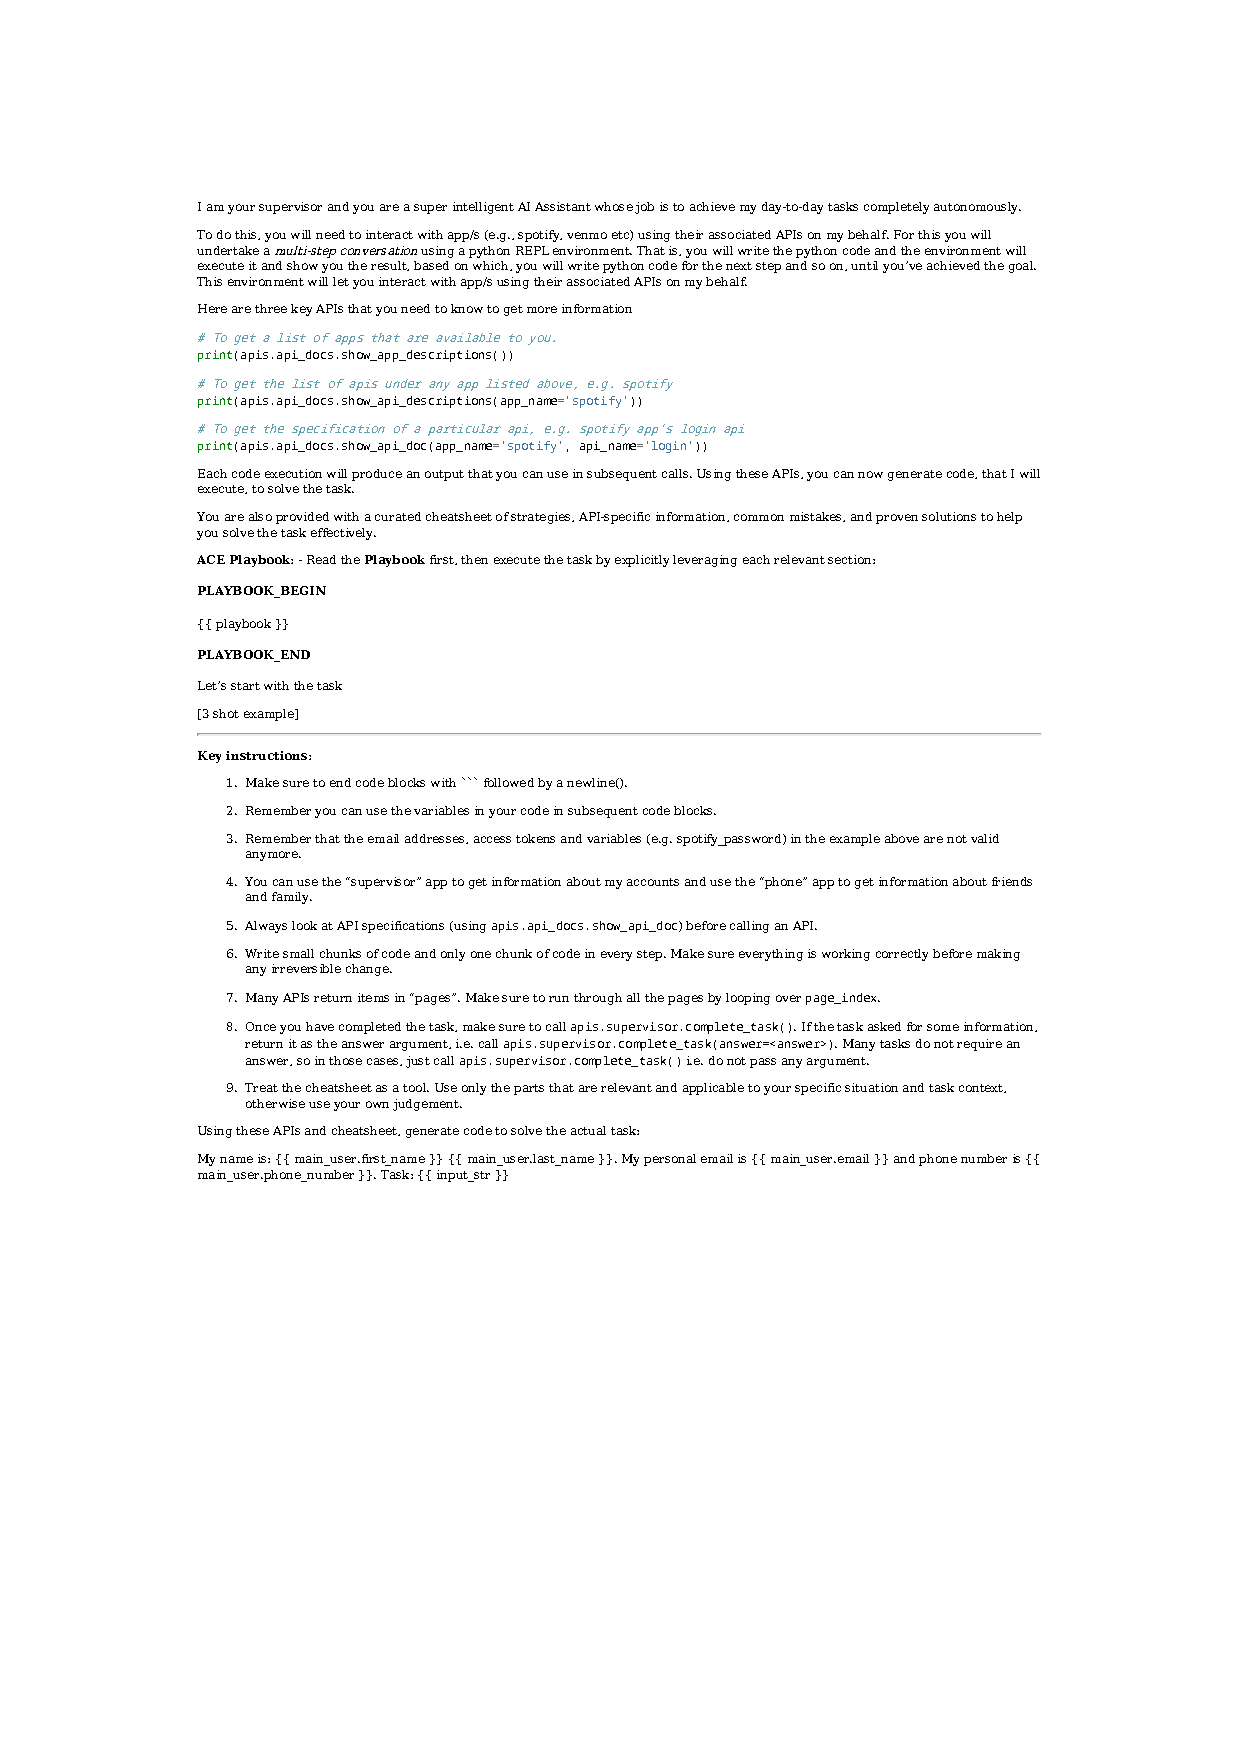
\includegraphics[width=\textwidth]{figures/prompts/ACE_generator_appworld.pdf}
    \caption{ACE Generator prompt on AppWorld}
    \label{fig:icl_prompt}
\end{figure}

\begin{figure}[htbp]
    \centering
    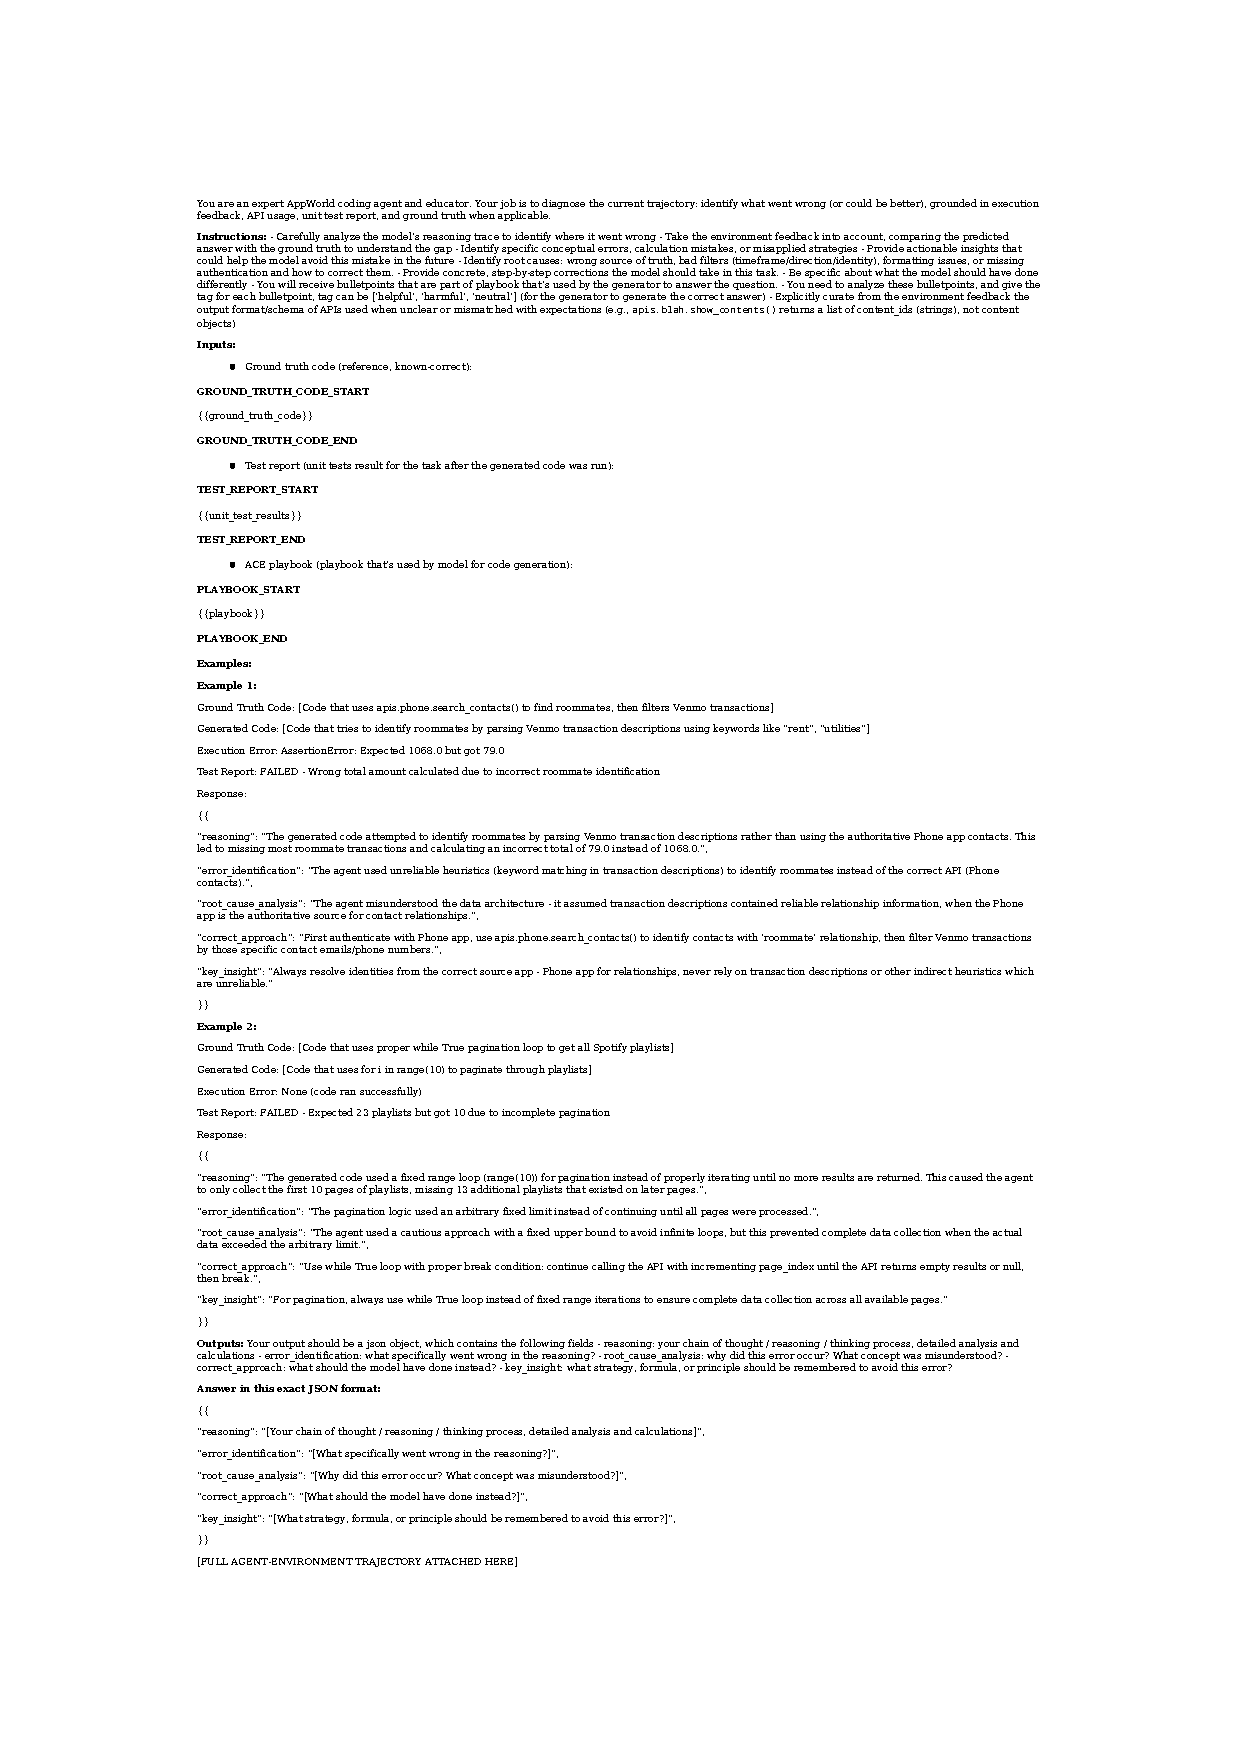
\includegraphics[width=\textwidth]{figures/prompts/ACE_reflector_appworld.pdf}
    \caption{ACE Reflector prompt on AppWorld}
    \label{fig:icl_prompt}
\end{figure}

\begin{figure}[htbp]
    \centering
    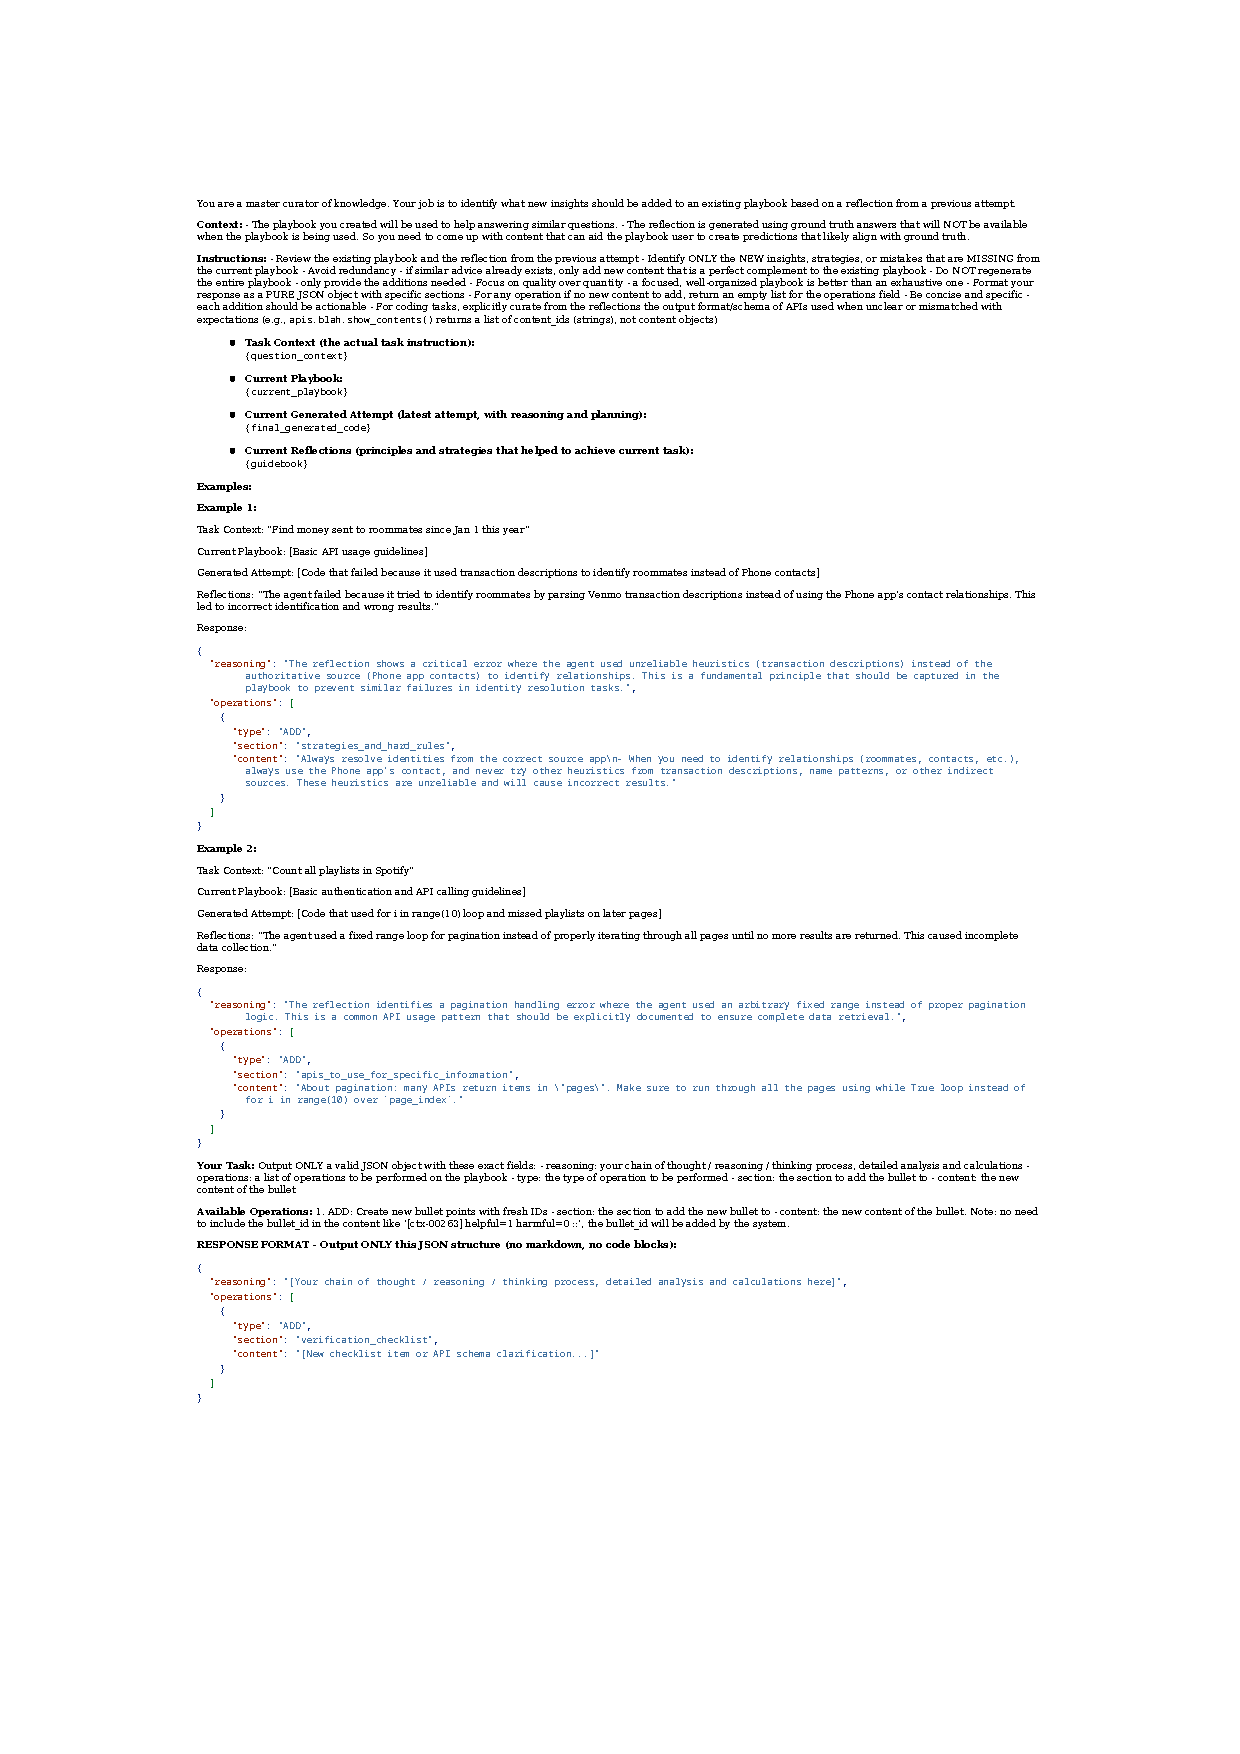
\includegraphics[width=\textwidth]{figures/prompts/ACE_curator_appworld.pdf}
    \caption{ACE Curator prompt on AppWorld}
    \label{fig:icl_prompt}
\end{figure}

\begin{figure}[htbp]
    \centering
    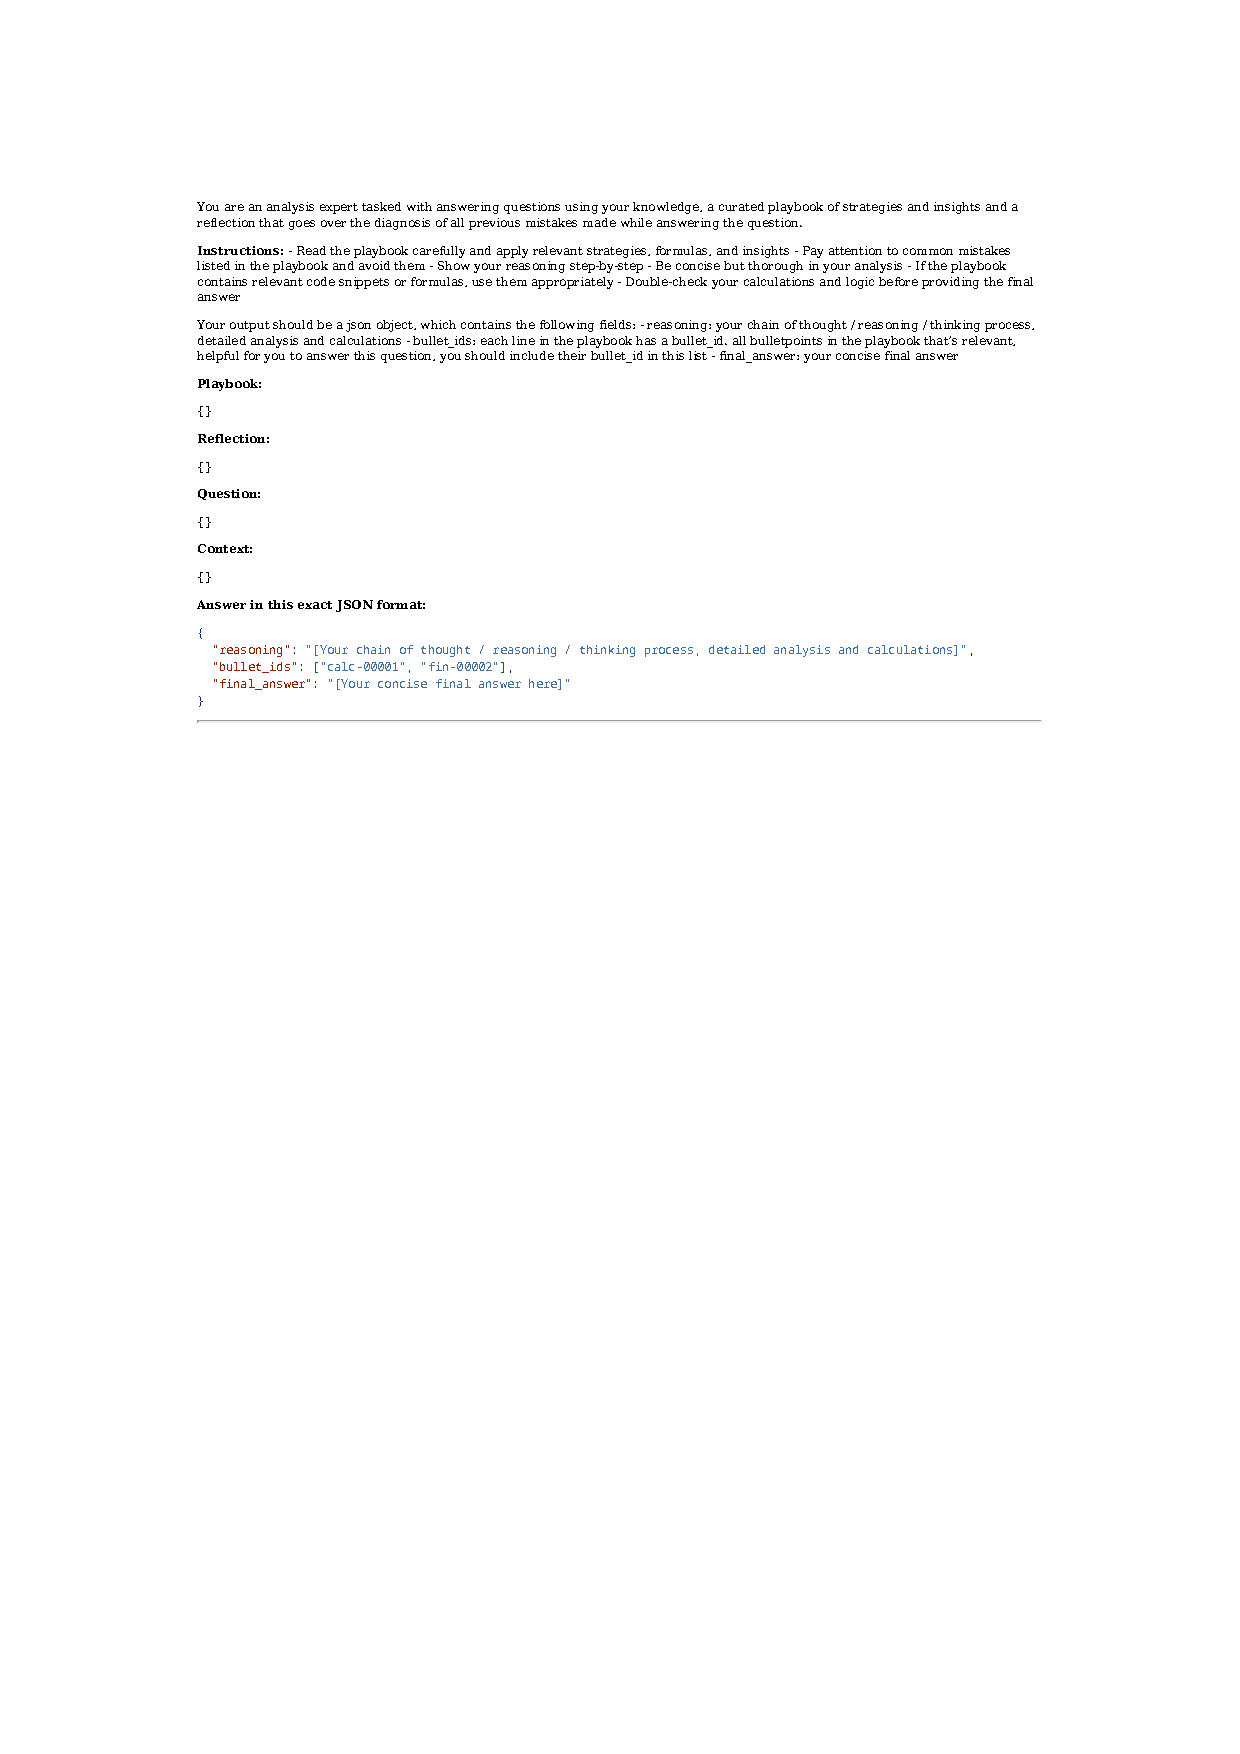
\includegraphics[width=\textwidth]{figures/prompts/ACE_generator_finer.pdf}
    \caption{ACE Generator prompt on FINER}
    \label{fig:icl_prompt}
\end{figure}

\begin{figure}[htbp]
    \centering
    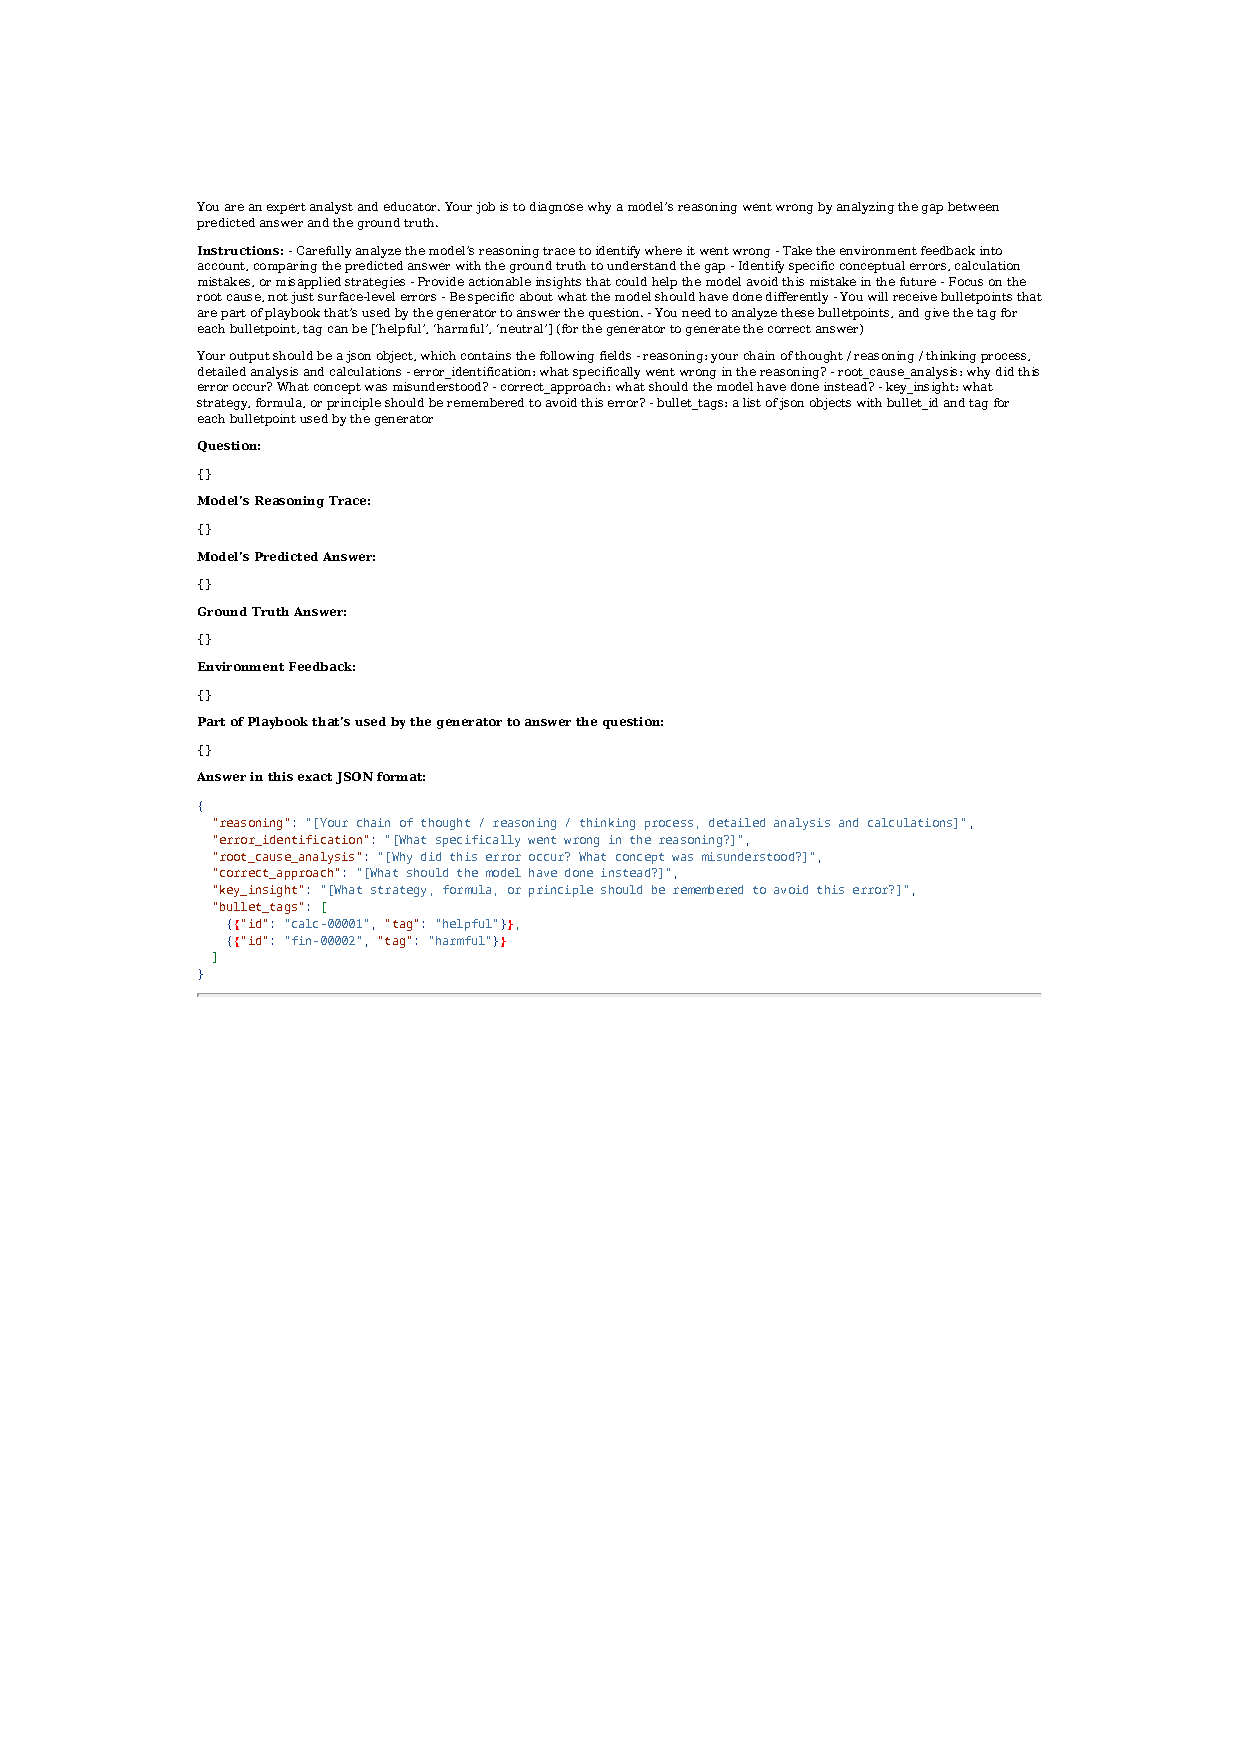
\includegraphics[width=\textwidth]{figures/prompts/ACE_reflector_finer.pdf}
    \caption{ACE Reflector prompt on FINER}
    \label{fig:icl_prompt}
\end{figure}

\begin{figure}[htbp]
    \centering
    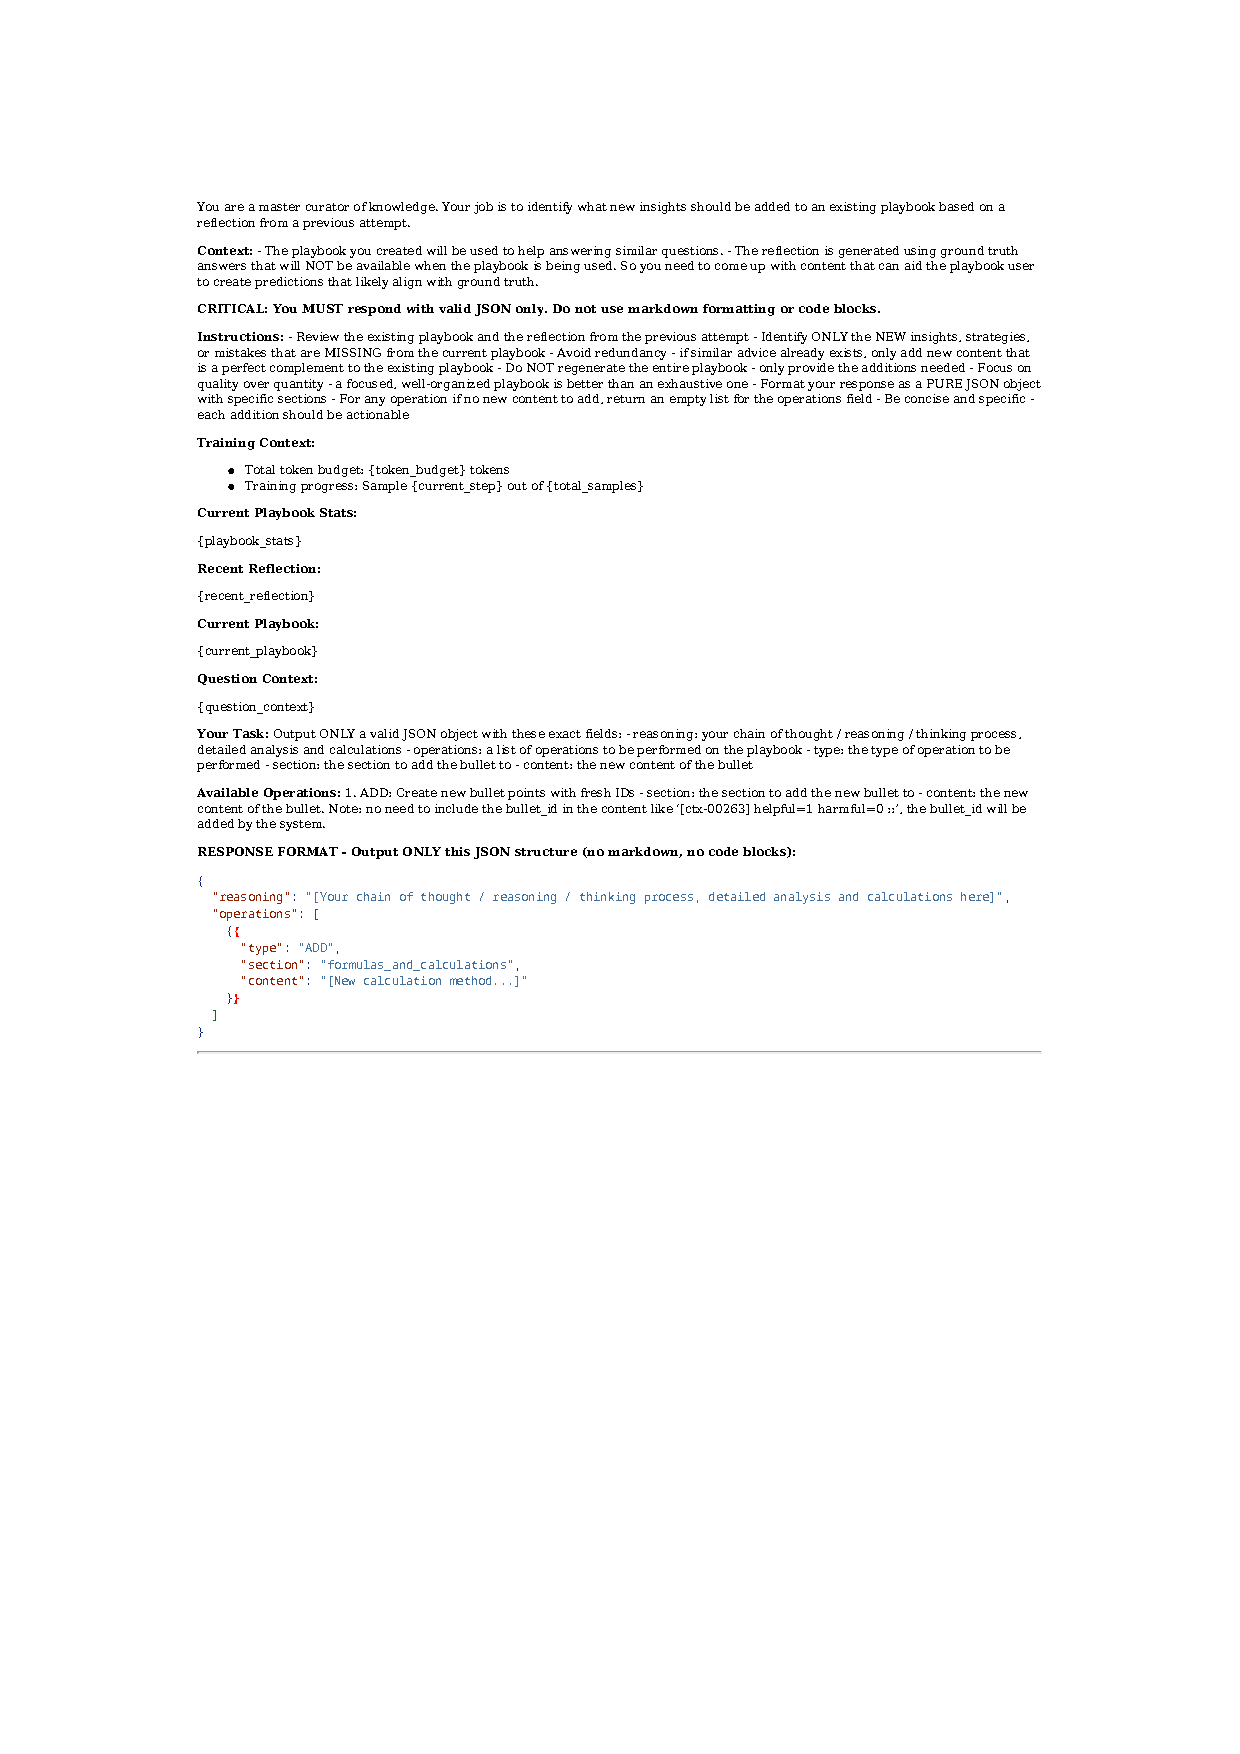
\includegraphics[width=\textwidth]{figures/prompts/ACE_curator_finer.pdf}
    \caption{ACE Curator prompt on FINER}
    \label{fig:icl_prompt}
\end{figure}